\documentclass[12pt]{article}
\usepackage[hmargin=2.0cm,vmargin=1cm]{geometry}
\usepackage[utf8]{inputenc}
\usepackage{graphicx}
\usepackage{float}
\usepackage{cite}
\usepackage{natbib}
\usepackage{amsmath}

\title{\begin{LARGE}
{The environmental effect on LAEs galaxies at the end of reionization $z\sim 6$}
\end{LARGE}}

\begin{document}
\maketitle

\section{Constants:}

In this section we define the constants used in this work.

\begin{table}[H]
\begin{center}
\begin{tabular}{c c c c}
\hline
Constant name & Symbol & Value & Units \\
\hline
\hline
Boltzmann  & $k_B$ & $1.3806488\times 10^-{23}$ & $[J/K]$ \\ 
Gravitational & $G$ & $6.67384\times 10^{-11}$ & $[\dfrac{m^3}{Kgs^2}]$\\
Mean molecular weight &$\mu_n$ & $0.59$ & $-$ \\
Proton mass & $m_p$ & $1.672621777\times 10^{-27}$ & [kg] \\
Slope parameter & $\beta$ & $0.4$ & $-$ \\
Matter density & $\Omega_m$ & $0.3089$ & $-$ \\ 
Barions density & $\Omega_B$ & $ 0.0455102$ & $-$ \\
Dark energy density & $\Omega_{\Lambda}$ & $0.6911$ & $-$ \\
Spatial curvature density& $\Omega_{k} $ & $-0.0023$ & $-$ \\
Hubble parameter & $H_0$ & $7.11449538303\times 10^{-41}$& $[1/s]$ \\
Solar mass &  $M_{\odot} $ & $1.9891\times 10^{30}$  & [kg] \\ 
%$m_p$
\hline
\end{tabular}
\end{center}
\end{table}

\section{Gas density profile:}\label{sec:rho}

Makino et al (1997) found an analytical expresion (Eq.8 in that paper) for the gas profile assuming that the gas
is isothermal and it is inside a DM halo with a NFW profile. They argue that this equation it's well approximated by 
the following profile:

\begin{equation}\label{eq:rhogr}
\rho_g(r) =  \dfrac{\rho_{g,0}A}{\left[ 1 + \left(\dfrac{r}{r_{c,eff}}\right)^2 \right]^{3\beta_{eff}/2}}
\end{equation}

Where $A(b) = -0.178b + 0.982$ and $\beta_{eff} = 0.9 b$\\

In order to compute $\rho_{g,0}$ we used Eq.14 in that paper:

\begin{equation}\label{eq:rhog0}
\rho_{g0} = \dfrac{f_{gas}\Omega_{b}\rho_{c0}\delta_{c}}{\Omega_0}e^{27b/2} \left [ Ln(1+c) - \dfrac{c}{1+c}  \right ] \left [ \int_0^c x^2(1+x)^{27b/2x} dx \right ]
\end{equation}

As an example for a DM  halo of $M = 1E12 M_{\odot}$ at $z=2$ and a concetrarion parameter of $c=3.75$
the gas profile is shown in Fig. \ref{fig:gp}

\begin{figure}\label{fig:gp}
\centering
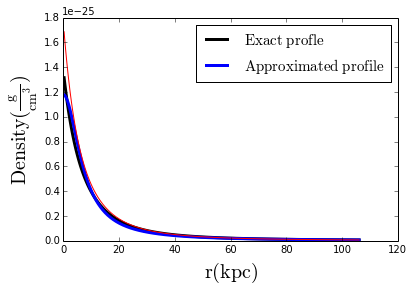
\includegraphics[scale=0.7]{../figures/gasprofile.png}
\caption{Gas density profile for a DM  halo of $M = 1E12 M_{\odot}$ at $z=2$ and a concetrarion parameter of $c=3.75$}
\end{figure} 


\section{Column density derivation:}\label{sec:NH}

In order to compute the column density of the gas profiles, we first
make an integral over the $z$ axys of the gas profile to get $N_{H}$i.e:

\begin{equation}
N_{H} = \int \limits_{-\infty}^{\infty}\rho_g(r)dz
\end{equation}

Where $r^2 = z^2 + b'^2$ and $b'$ is the impact parameter.
Changing variables from $z$ to $r$ we get:

\begin{equation}
N_{H} = \rho_{g0}A \int \limits_{-\infty}^{\infty} \dfrac{dz}{\left 
[ 1 + \left(\dfrac{r}{r_{c,eff}} \right)^2 \right]^{3\beta_{eff}/2}}
= \rho_{g0}A \int \limits_{b}^{\infty}\dfrac{r}{\sqrt{r^2 - b'^2}}\dfrac{dr}
{\left [ 1 + \left(\dfrac{r}{r_{c,eff}} \right)^2 \right]^{3\beta_{eff}/2}} 
\end{equation}

The result of the integral is:

\begin{equation}\label{eq:NH}
N_{H} = \rho_{g0} A\dfrac{\sqrt{\pi} (\dfrac{1}{r_c(M_h)^2})^{-3\beta_{eff}(M_h) /2} (b'^2 + r_c(M_h)^2)^{1/2 - 3\beta_{eff}(M_h)/2} \Gamma(-1/2 + 3\beta_{eff}/2) }{2 \Gamma(\dfrac{3\beta_{eff}(M_h)}{2})}  
\end{equation}

The $N_H$ for all the halo masses and for all the impact parameters would
be defined as:

\begin{equation}\label{eq:integral}
<N_H> = 4 \int \limits_0^{0.5} dx \int \limits_{0}^{0.5}dy \int 
\limits_{M_{Hmin}}^{M_{Hmax}} N_H(b, M_H)\xi(M_H)dM_H  
\end{equation}

Where the impact paremeter $b'^2 = x^2  + y^2$ and $M_{Hmin} = 1\times 10^4 
M_{\odot}$ and $M_{Hmax} = 1\times 10^{12}M_{\odot}$. And $\xi(M_H)= \dfrac{dn}
{dM_H}$. The dependence with the redshift is in the computation of $r_{vir}$ and
in the mass function.

In order to evaluate  Eq. \ref{eq:integral} we first make the integral over
the mass using the trapezoid method as follows:

\begin{equation}
\int \limits_{M_{HMin}}^{M_{HMax}} N_H(b, M_H)\xi(M_H)dM_H =  \sum_{0}^{1000}\Delta_M \left[ \dfrac{N_H(b, M_{H}+\Delta_M) \xi(M_{H + \Delta_M}) + N_H(b, M_{HM}\xi(M_{H}))}{2}\right]
\end{equation}

Which can be expressed as:

\begin{equation}
\begin{split}
\int \limits_{M_{HMin}}^{M_{HMax}} N_H(b, M_H)\xi(M_H)dM_H = \sum \limits_{0}^{1000}\Delta_{M} M_{\odot}  \dfrac{\rho_{g0} A(b) \sqrt{\pi} \Gamma(-\dfrac{1}{2} + \dfrac{3\beta}{2})}{4\Gamma{\dfrac{3\beta}{2}}} \\
\left[ \left( \dfrac{1}{r_c(M_{HMin})^2} \right)^{-3\beta/2} (b^2 + r_c(M_{Hmin})^2)^{1/2 - 3\beta/2} \xi(M_{Hmax})+ \\
 \left( \dfrac{1}{r_c(M_{HMax})^2} \right)^{-3\beta/2}(b^2 + r_c(M_{Hmax})^2)^{1/2 - 3\beta/2}\xi(M_{Hmin}) \right] 
\end{split}
\end{equation}

The average column density of a ray traced in a volume of $1Mpc^3$ at redshift $z=6$ is then given by:

\begin{equation}
<N_H> = 4 \rho_{g,0}A\int \limits_0^{0.5} dx \int \limits_{0}^{0.5}dy N_H(b) db = 1.68\times 10^{-42} \dfrac{g}{cm^3}
\end{equation}


\section{Neutral Hydrogen fraction $\eta$:}\label{sec:eta}

Following Rahmati et al 2013, we compute de neutral hydrogen fraction $\eta = n_{HI} / n_H$. We follow
the procedure implemented in the Appendix A in that paper.\\

\begin{equation}\label{eq:eta}
\eta = \dfrac{B - \sqrt{B^2 - 4AC}}{2A}
\end{equation}

Where $A$ , $B$ and $C$ are defined as: 

\begin{equation}
\begin{split}
A = \alpha_A + \Lambda_T \\
B = 2\alpha_A + \dfrac{\Gamma_{Phot}}{n_H} + \Lambda_T \\
C = \alpha_A
\end{split}
\end{equation}

where $\Lambda_T$, $\alpha_A$ and $\Gamma_{Phot}$ are defined as:

\begin{equation}
\Lambda_T = 1.1.7 \times 10 ^{-10} \dfrac{T^{1/2} exp(-157809/T)}{1 + \sqrt(T/10^5)} cm^3 s^{-1}
\end{equation}


\begin{equation}
\alpha_A = 1.269 \times 10 ^{-13} \dfrac{\lambda^{1.503}}{(1 + (\lambda / 0.522)^{0.47} )^{1.923}} cm^{3} s^{-1}
\end{equation}

where $\lambda = 315614 / T$. 

\begin{equation}
\Gamma_{Phot} = \Gamma_{UVB} \left(  0.98\left[ 1 + \left( \dfrac{n_H}{n_{H, SSh}} \right)^{1.64}  \right]^{-2.28} + 0.02 \left[ 1 + \dfrac{n_H}{n_{H,SSh}} \right]^{-0.84}   \right) 
\end{equation}

The up of Fig.\ref{fig:eta} shows how neutral Hydrogen fraction changes for diferent hydrogen densities, 
for different Halo Mass.
While the bottom figure shows the bahaviour of $\eta$ as a function of the temperature $T$. The blue 
line is for a Hydrogen density $n_H = 0.01 cm^{-3}$ which is above the selfshielding density limit, 
while the black line is for $n_H  = 0.001 cm^{-3}$.

\begin{figure}[H]\label{fig:eta}
\centering
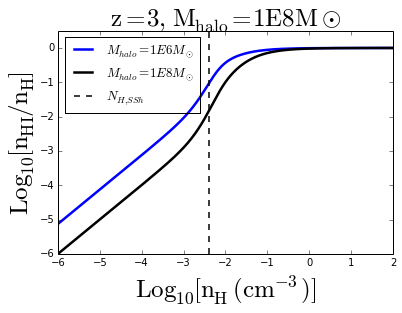
\includegraphics[scale=0.7]{../figures/etavsnh.png}
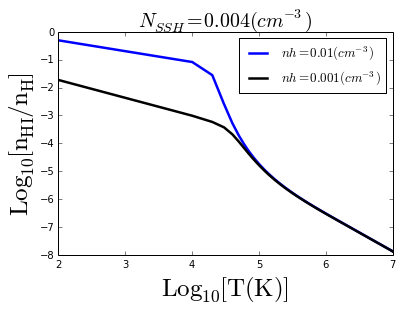
\includegraphics[scale=0.7]{../figures/etavsT.png}
\caption{(Up) }
\end{figure}

\section{Neutral Hydrogen density profile}\label{sec:NHI}

In ordert to study the effect of the environment in LAEs we are interested in the neutral Hydrogen. 
To this aim we want to derive the neutral Hydrogen gas profile using Makino's profile alongside 
the neutral hydrogen fraction derived in the previous section. 

The first step here is to find the Hydrogen density $n_H$ from the $\rho$ this is related by $n_H = \rho / m_p$, 
this profile is shown in Fig.\ref{fig:nhvsr}.

\begin{figure}[H]\label{fig:nhvsr}
\centering
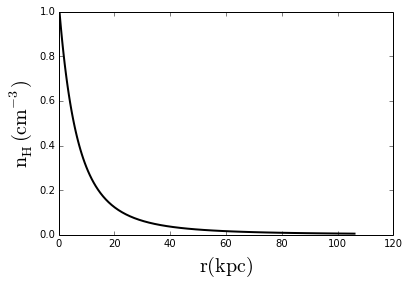
\includegraphics[scale=0.7]{../figures/nhvsr.png}
\end{figure} 

With this density $n_H$ we compute the neutral Hydrogen fraction $\eta$ as function of $r$, Fig.\ref{fig:etavsr}
show the fraction of neutral Hydrogen inside a DM halo of mass $M=10^8 M_{\odot}$ at $z=6$ with $r_{vir} = 1.67 Kpc$.

\begin{figure}[H]\label{fig:etavsr}
\centering
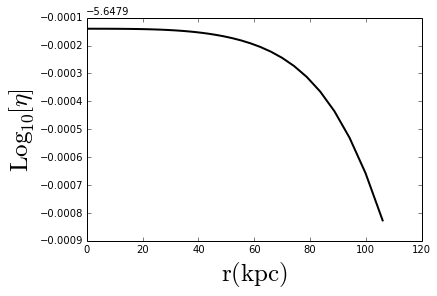
\includegraphics[scale=0.7]{../figures/etavsr.png}
\end{figure}

With this information we can compute the Neutral Hydrogen profile corresponding to this DM halo by multplying
$n_{HI}(r) = \eta(r) n_{H}(r)$, this is shown in Fig.\ref{fig:nhivsr}.

\begin{figure}[H]\label{fig:nhivsr}
\centering
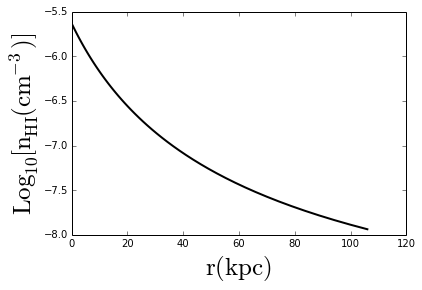
\includegraphics[scale=0.7]{../figures/nhivsr.png}
\end{figure}  


\section{Numerical Approch}

We use the results of a DM only simulation Illustris1 with the aim 
of studing how the environment affects the absorption of 
Ly$\alpha$ radiation at $z\sim6$. We chose emitters halos to be 
those in a range of mass  $7 \times 10^{10} - 2 \times 10^{11}$, this 
halos have different environments (\textbf{Make a plot of this}).
We then trace rays of Ly$\alpha$ photons in random dierections, and we derive
the gas properties of those halos that interact with the ray 
implementing the equations described in \S \ref{sec:rho}, 
\S \ref{sec:NH},\S \ref{sec:eta}.\S \ref{sec:NHI}. Then we sum the column 
density of every Ly$\alpha$ ray. In the following subsections we describe 
these steps in detail.  

\subsection{Dark Matter halo catalogue}

We use the public available data from the Illustris simulation, in particular we use 
the Illustis1-dark catalogue. This is a simulation of $1820^3$ dark matter particles
with a mass of $m_{DM}=6.3 \times 10^6 M_{\odot}$ in a box of $L=106.5 Mpc$. We use 
the data of halos at $z = 6.01$. 

\subsection{Ray tracing}

We select emitter galaxies in the range of $7 \times 10^{10} - 2 \times 10^{11}$.
There are N halos in this mass range in the simulation. All these halos
are in different environmets.  

After selecting randomly an emitter we follow the trayectory of a Ly$\alpha$ photon 
in a random direction and for ray length of $10 Mpc$. In $10 Mpc$ a Ly$\alpha$ would 
have a $\Delta_z$ of: 

We then compute the impact parameter $b$ between the ray and all the halos that could
possibly absorbe the photons, we select those halos in which the condition $b<R_{vir}$ 
is ensured, those halos would be the absorbers. 

\textbf{How many absorbers have each ray, try to visualize this}

\subsection{Colulmn density properties and Environment}

We compute the density profiles of using Eq.\ref{eq:rhogr}, the
we compute the column density using Eq.\ref{eq:NH}. Then we compute
the fraction of neutral column density $n_{HI}$ using Eq.\ref{eq:eta}

We define the environment of a emitter halo as:

\begin{equation}
\Delta_3  = \bar{r}^3 \left( \dfrac{1}{r^3} - \dfrac{1}{\bar{r}^3} \right)
\end{equation}

Where if $\Delta_3 < 0 $ we say that the halo is in an overdense enviroment while
if $\Delta_3 > 0 $ the halo is in an underdense environment.

\section{Results}

\begin{figure}[H]
\centering
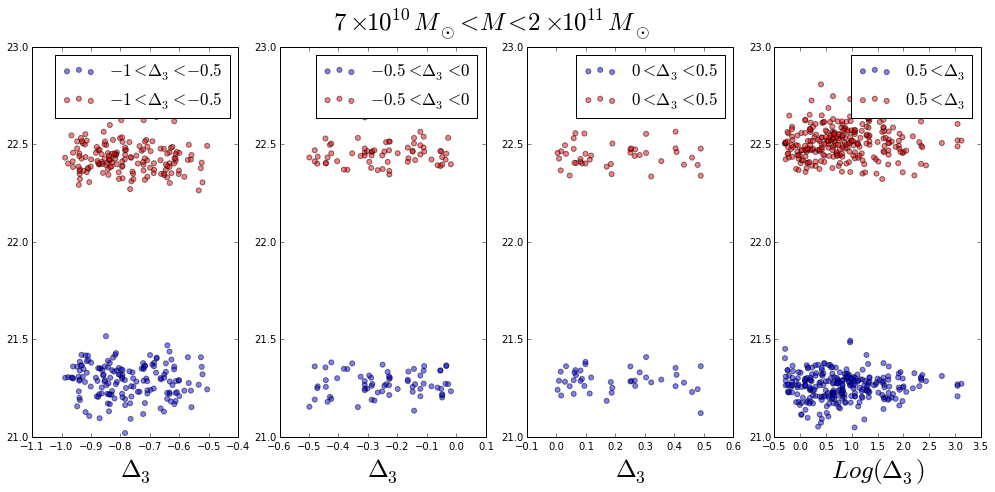
\includegraphics[scale=0.4]{../figures/NHI.png}
\end{figure}

\begin{figure}[H]
\centering
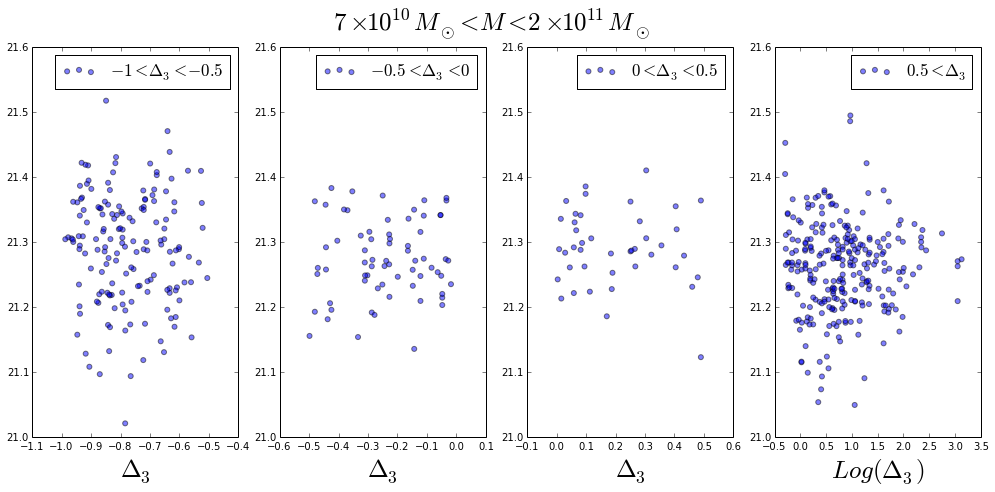
\includegraphics[scale=0.4]{../figures/NHIvsD3.png}
\end{figure}

\end{document}
